\section{Results} \prasannnote{TODO more descriptive section names}
% \sewonnote{Is this section about validating \cname? Rather, I think it's about connecting task complexity (\cname) and model complexity.}

% We here walk through our design decisions with a motivating task. We'll show how architectural decisions interact with task structure and scale, before getting into our main results (Section~\ref{sec:taskcompresults}). 

We previously investigated how improving learning dynamics can be helpful for different approaches on higher \cname tasks, especially with mask mixing. This isolates the role of learning signal, \textit{but does this overcome architectural limitations of chunked attention}? We measure performance over increasing corpus sizes to connect \cname and method complexity. 


%We report in Table~\ref{tab:mask-mix-suite} an exemplar set of settings where, when comparing the inclusion vs the exclusion of mask mixing, we see notable gains. Overall, mask mixing seems to be a consistent trick to aid learning in our settings: allowing for better performance with higher inference-scalability. .



% That said, \emph{following our application of mask mixing to our main results} (Figure~\ref{fig:sec5-cross-task}), we note that the fundamental gap from \cname remains even with mask mixing, suggesting that while learning signal issues can be addressed via analysis of learning dynamics, addressing gaps in complexity is a longer-term problem. 





% \sewonnote{Setup is mixed in this section. Clearly separate the setup to the earlier section, so that this section can solely focus on results.}
\subsection{Main Results: \cname Method Scaling}

\label{sec:taskcompresults}
% \subsection{Main Results: Relationship Between \cname and Method Complexity}

\prasann{All this text is outdated}

\begin{figure}[t]
\centering
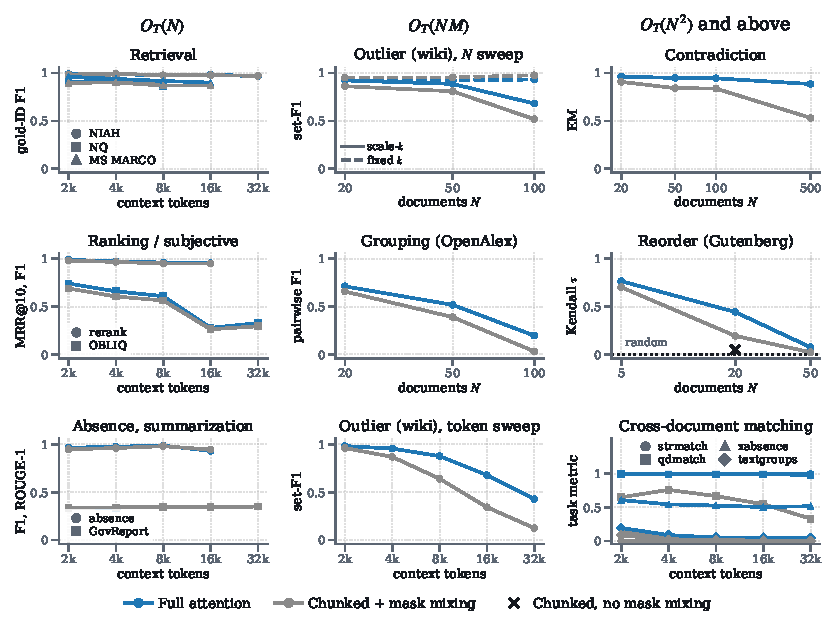
\includegraphics[width=\textwidth]{figures/fig4_cross_task.pdf}
\caption{\emph{Cross-task scaling of full vs.\ chunked attention (with our mask mixing technique).} Each panel plots corpus size on the x-axis---either the document count $N$ or the context token budget, which scales $N$ per task---against the task-specific metric, for 16 settings spanning the suite. Columns are \cname{} classes. \textbf{\boldmath \ctc{N} tasks have a small gap throughout} (left column, 7 tasks: the full-chunked gap never exceeds $0.07$ at any budget, and chunked is \emph{ahead} on NQ and GovReport). Meanwhile, for Outlier scale-$k$, Grouping and Contradiction \textbf{the size of the full vs.\ chunked gap increases by 2.7x, 3.1x and 6.4x respectively} between the smallest and largest corpus; carrying Outlier out to a 32k budget (middle column, bottom) widens it \textbf{15x}, from $0.02$ to $0.30$. On the Reorder task chunked hits random while standard stays above random, hence why the gap can't widen. For the outlier task, we ablate keeping $M$ constant (dashed lines), and \textbf{find it behaves like an \ctc{N} task} in that setting. Sample non-mixing run (X) shown on reorder task. The high-\cname{} column also shows two distinct chunked failures: \emph{graceful decay} (qdmatch, xabsence, textgroups) and \emph{collapse} from the first rung (strmatch, where chunking makes exact cross-document string matching structurally impossible). All panels are Qwen3.5-4B except Reorder (9B); 500 eval examples per rung, except contradiction (488, the full held-out set) and OBLIQ (\textbf{126 only}, SE $\pm0.045$). \prasann{TODO non-maskmix lines beyond the single reorder X point}}
\label{fig:sec5-cross-task}
\end{figure}
\autonote{Regenerated: 9 panels, +5 from the 4B suite. Outlier/Grouping/Contradiction/Reorder unchanged; old NQ + HPQA (0.8B) panels dropped --- prose below still cites HPQA. 6.5x recomputed to 6.4x.}



% \prasannnote{RYAN: Thicker lines maybe, maybe figures are a little small? Fix grouping x-axis }

% We here ask \textbf{how do tasks with different \cname requirements interact with different complexity of computation}? Performance gaps at scale are key here: if our hypothesis is true, then we'll expect on \cmc{N} for chunked and standard attention to perform high / similarly. For \ctc{NM} tasks we may expect the gap to widen as both N and M increase (if M doesn't increase then it should behave like an \ctc{N} task). And for \ctc{N^2} tasks the gap should widen even more with greater contexts.

\paragraph{Results}  We plot results in Figure~\ref{fig:sec5-cross-task} with several points of context length (x-axis) vs task performance (y-axis) of systems trained in-domain on those contexts. In each setting, the relative increase in gaps aligns with our \cname categorization. Up to 200 documents per context, both \ctc{N} tasks show very similar full and chunked attention performance, with low degradation with scale (e.g. HPQA stays above 0.75 F1 until the end, and the gap between chunked and standard remains nearly identical). On our \ctc{NM} tasks, there's a consistently widening gap between full and chunked attention (\textbf{roughly 3x gap size increase} between k=20 and k=100). This is not true, however, if we hold constant the number of categories ($M$) with increasing $N$ (represented in the figure by the dotted lines); in this case, the Outlier task behaves similarly to HPQA. Scaling $M$ alongside $N$ makes the task harder---supporting the \ctc{NM} categorization. Lastly, the contradiction and reorder tasks (\ctc{N^2}) \emph{both see large widening gaps} emerge between chunked and standard at greater scale. \textbf{Reorder's gap only seems smaller at N=50 as chunked hits random performance} (whereas standard doesn't).  \emph{Despite using mask mixing, chunked attention remains unable to keep up with growing corpora across high \boldmath \cname tasks}.

%\amandanote{maybe drop this (sentence about mask mixing) now that mask mixing is explained earlier? it no longer needs to be in this figure too imo}


\subsection{The Roles of Task Sparsity and Model Scale}

\label{sec:sparsityscaleresults}

We'll here motivate some of the decisions of the above experiment, while also shedding greater insight into how sparsity and model scale play a role in scaling on the high-\cname contradiction task.



\begin{figure}[t]

    \centering
    \begin{minipage}{0.48\textwidth}
        \centering
        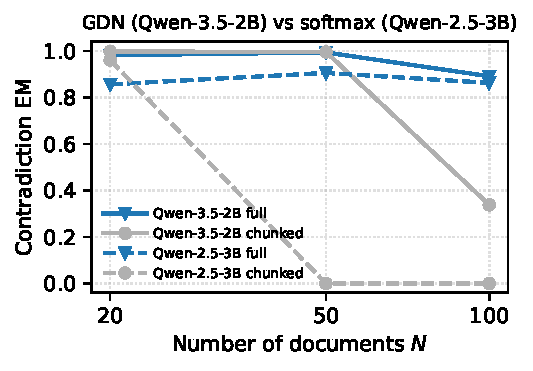
\includegraphics[width=\textwidth]{figures/section4_gdn.pdf}\\
        \small (a) Qwen-3.5 vs Qwen-2.5
    \end{minipage}
    \hfill
    \begin{minipage}{0.48\textwidth}
        \centering
        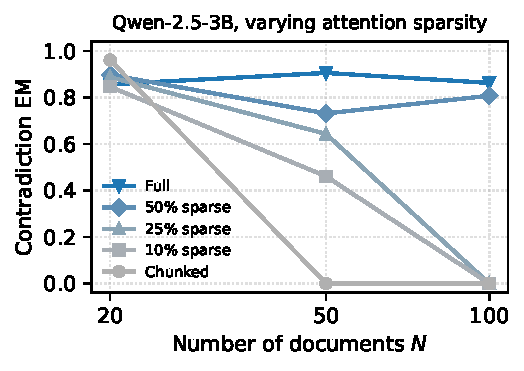
\includegraphics[width=\textwidth]{figures/section4_sparsity.pdf}\\
        \small (b) Role of sparsity (Qwen-2.5-3B)
    \end{minipage}
\vspace{-0.2em}
\caption{\emph{Contradiction-task scaling.} \textbf{(a)} Qwen-3.5-2B, with 75\% GDN layers, has better chunked scaling than Qwen-2.5-3B (full attention). \prasann{TODO 2-3 more model families} \textbf{(b)} Role of attention sparsity: \textbf{greater sparsity leads to faster degradation} with scale.}

\label{fig:sparsityscale}

\end{figure}


\begin{wrapfigure}{r}{0.5\textwidth}
    \centering
    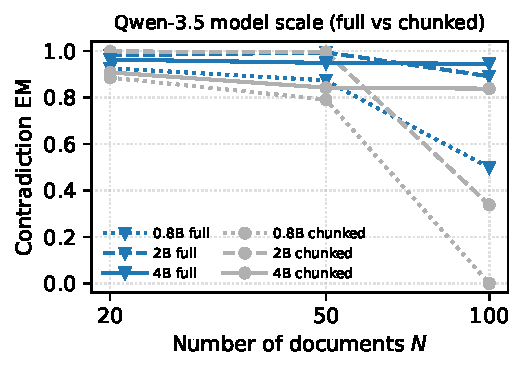
\includegraphics[width=0.5\textwidth]{figures/section4_scale.pdf}
    \caption{\emph{Model scale (Qwen-3.5).} Increasing model scale within the Qwen-3.5 family (solid: 4B, dashed: 2B, dotted: 0.8B) pushes back the point at which the chunked variant degrades, but \textbf{small full attention models can beat larger chunked attn}.}
    \label{fig:modelscale}
    \vspace{-1em}
\end{wrapfigure}

\textbf{Alternative Architectures} To test the role of base model, we compare Qwen-3.5, which uses 75\% GDN layers with Qwen-2.5 \citep{qwen2.5}, with full standard attention (no GDN layers). For both, to compare \cmc{N^2} and \cmc{N}, we use masks to convert just the standard attention layers to chunked attention. In Figure~\ref{fig:sparsityscale} (a), notice how, despite being smaller, \textbf{Qwen-3.5-2B chunked shows degradation later than Qwen-2.5-3B}. While this may be partially attributed to Qwen-3.5 being a stronger base model, this provides intial evidence that GDN approaches are not inherently less suited to such tasks (in fact, they may be better). As a result, we use Qwen-3.5 for most of our investigation. 


\textbf{Sparsity} We see above that \cmc{N} and \cmc{N^2} computation show gaps on high-\cname tasks, but what about cheaper methods within \cmc{N^2} like random document sparsity (recall Figure~\ref{fig:masks})? To test this, in Figure~\ref{fig:sparsityscale} (b), for $N=20, 50, 100$, we plot the results of training and evaluation for a Qwen-2.5-3B model (which uses full standard attention and is most affected by the sparse masks), with sparsity $\alpha = 0$ (chunked) $10\%, 25\%, 50\%$, and $100\%$ (full attention).  The pattern is clear: full attention approaches scale gracefully even over large contexts, but \textbf{increased sparsity corresponds to much greater scaling degradation}. Given that the contradiction task is \ctc{N^2} \cname, this aligns with the expectation that reducing computation with respect to scale will damage performance. 




% \begin{figure}[t]
%     \centering
%     \begin{minipage}{0.32\textwidth}
%         \centering
%         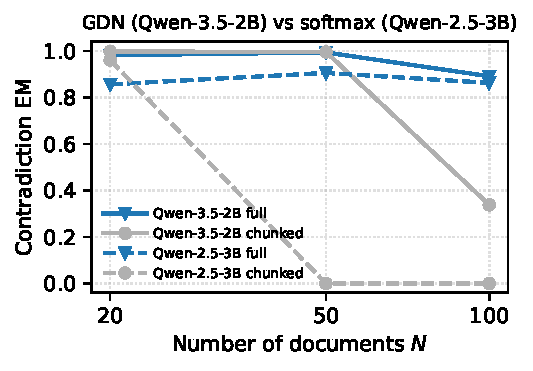
\includegraphics[width=\textwidth]{figures/section4_gdn.pdf}\\
%         \small (a) Qwen-3.5 vs Qwen-2.5
%     \end{minipage}
%     \hfill
%     \begin{minipage}{0.32\textwidth}
%         \centering
%         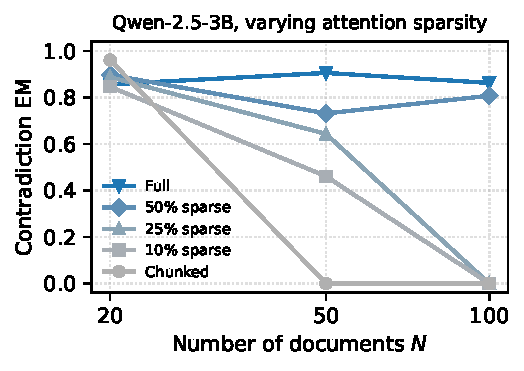
\includegraphics[width=\textwidth]{figures/section4_sparsity.pdf}\\
%         \small (b) Role of sparsity (Qwen-2.5-3B)
%     \end{minipage}
%     \hfill
%     \begin{minipage}{0.32\textwidth}
%         \centering
%         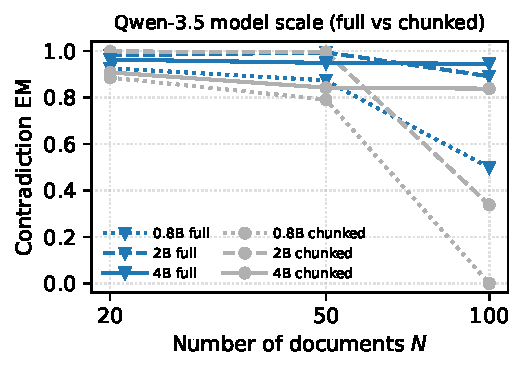
\includegraphics[width=\textwidth]{figures/section4_scale.pdf}\\
%         \small (c) Model scale (Qwen-3.5)
%     \end{minipage}
% \vspace{-0.5em}
% \caption{\textbf{Contradiction-task scaling} \textbf{(a)} Qwen-3.5-2B, with 75\% GDN layers, has better chunked scaling than Qwen-2.5-3B (full attention). \textbf{(b)} Role of attention sparsity: \textbf{greater sparsity leads to faster degradation} with scale.  \textbf{(c)} Increasing model scale within the Qwen-3.5 family (black: 4B, blue: 2B, gray: 0.8B) pushes back the point at which the chunked variant degrades, but \textbf{small full attn models can beat larger chunked attn models}.} 

% \label{fig:sparsityscale}
% \end{figure}



% \amandanote{Not a before-wednesday problem, but we should compare olmo3 7b to olmo3 hybrid 7b to make this argument more cleanly--- they're the same size + data!} \prasannnote{Ohh that's a good idea! }

\textbf{Model Scale} We saw earlier that even differences within $N^2$ computation (different sparse masks) affected task scaling. Here we test the effects of \emph{model size} as another axis to vary computation. We vary model scale for a few sizes of Qwen-3.5 models (0.8B, 2B, 4B) to examine how model scale affects degradation patterns, in particular for chunked attention. As shown in Figure~\ref{fig:modelscale} , we note that increasing model scale pushes back chunked degradation at longer contexts, which makes sense as the query / answer tokens have greater capacity for computation, and the GDN state is larger. Interestingly, however, we also find that \textbf{smaller models with standard attention can often go further than larger models with chunked attention}, validating the importance of scaling method computation alongside \cname for larger-scale versions of tasks. This is even more pronounced for non-GDN attention models: while not shown in the figure, we found chunked Qwen-2.5-14B at N=50 to in fact lag behind standard Qwen-2.5-3B despite 4.5x more parameters.


\subsection{Analyzing Atomic Operations}

\prasann{TODO some analysis of modified version of xabsence, other setting to show some different trend via more difficult atomic operations}

% \textbf{Full Attention} Of course, the most expressive approach currently available (full self-attention), is the most expressive, and so in some sense we are bound to tasks which can be reduced to the computational \cmc{N^2} of full attention. The drawback is that this is prohibitively expensive on truly large corpora.

% \textbf{Random Attention Masks} Chunked attention is cheap, but largely forgoes the ability to handle cross-document relationships. One solution is to have each token attend to a random percentage (e.g. 25\%) of prior document tokens (random sparse attention). This is \cmc{N^2}, but with a lower base computation can still be cheaper than full attention.

% \textbf{Chunked Attention} In our simplest chunked attention setting, individual documents can attend within themselves (e.g. Doc 1 content can attend causally to itself, see mask in Figure~TODO), but document tokens can \textbf{not} attend to any other documents. Documents can be encoded cheaply in parallel (thus \cmc{N} computation) but it completely relies on query / cot / answer tokens to handle aggregation and cross-document relations. We implement this via a causal attention mask (see Figure~TODO). 

% \textbf{}{Linear Attention Variants} 

% \paragraph{Random Attention Masks / Anchor Tokens} The above approaches generally lack good ways to build multi-document representations. One potential solution is to have each token attend to a random subset of prior document tokens (random sparse attention), or have dedicated tokens in each document (\emph{anchor tokens}) which all future tokens can attend to, allowing different documents to attend to each other without the cost of full attention, but the overall cross-document attention is much lower, and so these approaches may not learn successfully.



% \prasannnote{We may want to make sure to get good literature coverage. I think we may have it but could be good to confirm}


% \subsection{An Initial Test}

% We evaluate the contradiction task at context size N=20, 50, and 100 with 3 claims, a smaller setting, to get an initial sense of (note in the next section we will examine larger context sizes). Based on some iteration (TODO Appendix), we compare the case of both using a chain of thought which heavily enumerates all documents, and a no-CoT case. We evaluate various attention mechanisms, from chunked to full attention, at varying levels of sparsity (e.g. random, document window sparsity at 5, 25, and 50 percent). Note that retrieval baseline performance on this task is inherently random.

% \paragraph{Results} We plot sparsity of different approaches and models vs performance on the task in Figure~TODO (note that all of these were trained and evaluated on the same in-domain data). We find that without the CoT, even at the 20 claim scale (500 tokens), models struggle to learn this task well without full attention. \prasann{TODO get / put in more results in between pure chunked and full attn}. With the CoT, things are a bit better, but standard attention seems to improve similarly if not more than sparse variants as a function of the sparsity. \prasann{One potential risk is that "you just haven't trained on enough data to overcome OODness of new attention mask", so we should probably select 1-2 runs to run at really large scale to sanity check this (though I think from looking at the loss curves I think we should be fine here)}

% Overall, in particular when taking in the relationship between model scale and various attention types that we examine, we conclude that there seems to be a relationship between how much computation different approaches provide, and the corresponding performance. \prasann{Hmm I wonder if there's a single "computation" number which we could plot and get a clean performance line for within model family...}